\section{Results and Discussion}


Through tens of thousands experiments across many signal-processing techniques (\textit{i.e.}, defences), random states, learning rates, model architectures, and attack configurations, we show that model defences generally fail to outperform the undefended model in either the benign or adversarial contexts --- regardless of configuration. Also, that the adversarial failure rate gains of larger ResNet configurations are driven by response time rather than true robustness; that these gains are dwarfed by the increase in training time; and that AFT models are a powerful tool for comparing model architectures and examining the effects of covariates. In the section below, we display and discuss the results for the CIFAR100, CIFAR10, and MNIST datasets for all attacks and defences.

\subsection{Benign and Adversarial Accuracy}
Figure~\ref{fig:accuracies} depicts the benign and adversarial accuracies across the various attacks and defences. We can clearly see that no defence consistently outperforms the undefended (control) model in either the benign (top) or adversarial context (middle). We also see that for all defences, we can find at least one configuration with arbitrarily high accuracy, though finding it might involve an expensive hyperparameter search as evidenced by the large variance (see top plot of Figure~\ref{fig:accuracies}). Likewise, the adversarial accuracy benefits greatly from model tuning, but that attacks are still effective on roughly 75\% of samples in the best case for most attacks (see middle plot of Figure~\ref{fig:accuracies}). Despite varying methods and computational costs, the attacks seem to be more or less equally effective with respect to adversarial accuracy (see bottom plot of Figure~\ref{fig:accuracies}).

\label{results}
\begin{figure}[!ht]
\centering
\begin{subfigure}
    \centering
    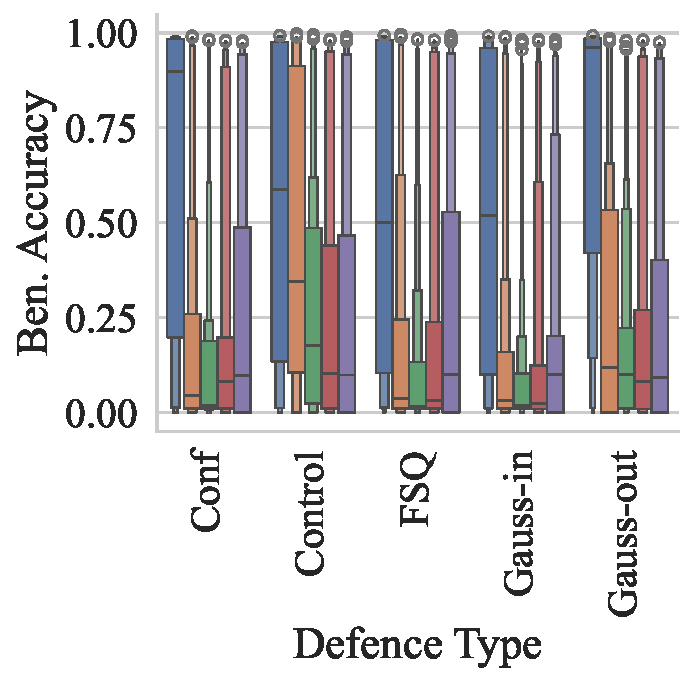
\includegraphics[trim={7pt 10pt 20pt 0pt},clip,width=.40\textwidth]{plots/ben_accuracy_vs_defence_type.pdf}
\end{subfigure}
\begin{subfigure}
    \centering
    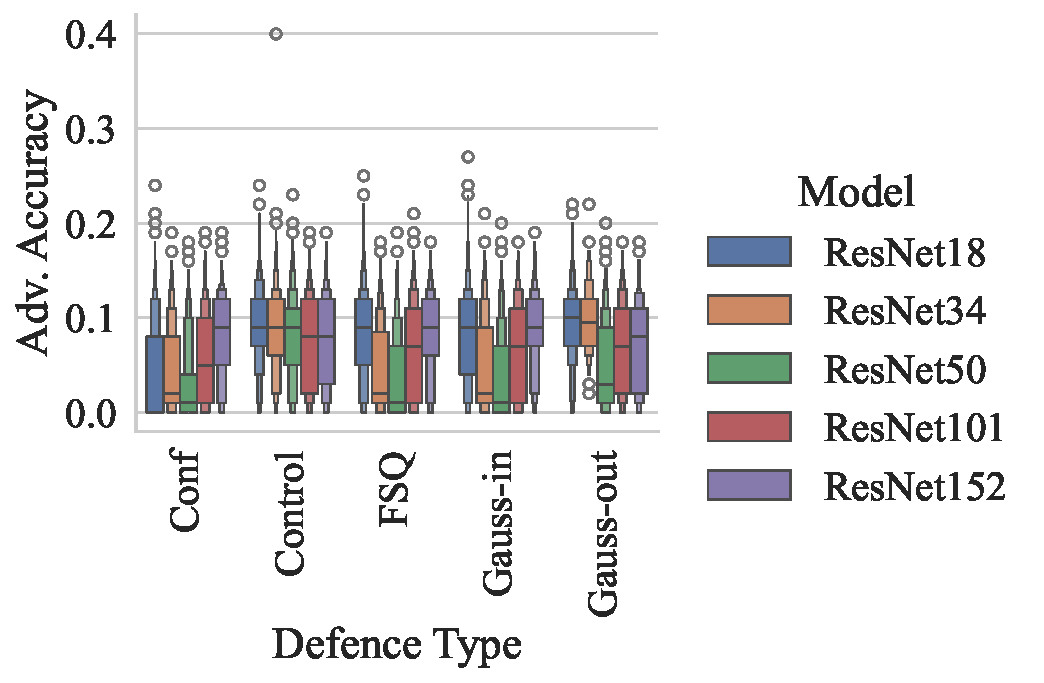
\includegraphics[trim={7pt 10pt 20pt 0pt},clip,width=.40\textwidth]{plots/adv_accuracy_vs_defence_type.pdf}
\end{subfigure}
\begin{subfigure}
    \centering
    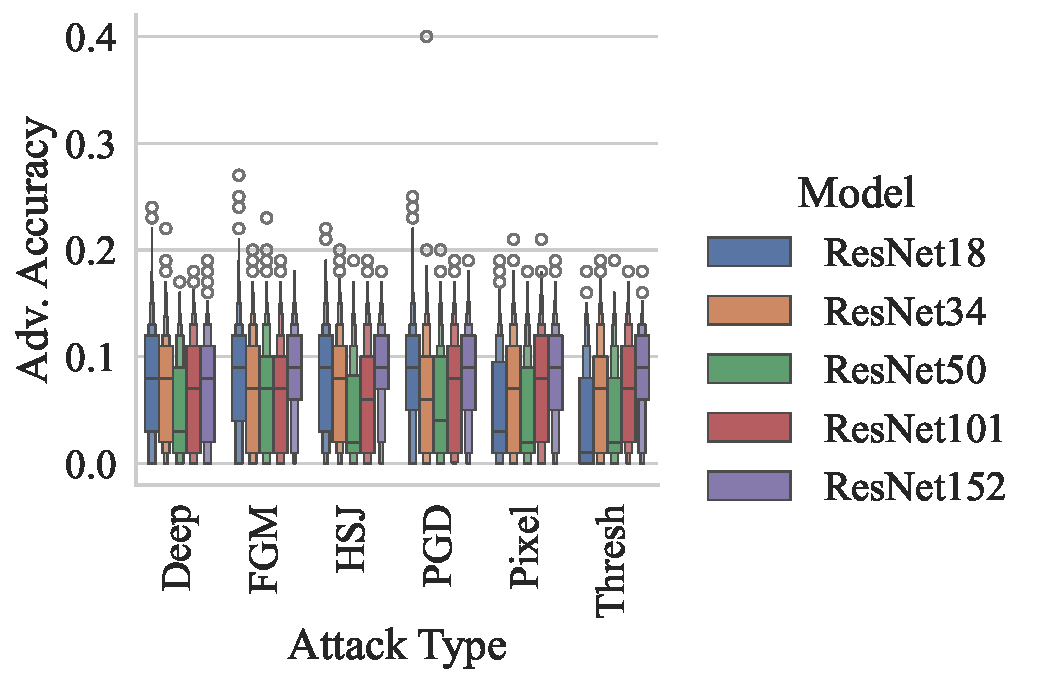
\includegraphics[trim={7pt 10pt 20pt 0pt},clip,width=.40\textwidth]{plots/adv_accuracy_vs_attack_type.pdf}
\end{subfigure}
\caption{The adversarial accuracy across various attacks pictured on the first axis and outlined in Section~\ref{attacks}. The error bars reflect 95\% confidence intervals for the adversarial accuracy across all examined samples. The violin plots reflect 95\% confidence intervals for each tuned hyperparameter combination. Outliers are indicated with a circle.}
\label{fig:accuracies}
\end{figure}

\subsection{AFT Models}

\begin{table*}[!ht]
\centering
\begin{tabular}{lllrrrrrr}
\toprule
 & AIC & BIC & Concordance & Test Concordance & ICI & Test ICI & E50 & Test E50 \\
\midrule
Cox & -- & -- & 0.92 & 0.92 & 0.06 & 0.27 & 0.04 & 0.09 \\
Gamma & -- & -- & 0.51 & 0.52 & 0.29 & -- & 0.24 & -- \\
Weibull & 9.05e+04 & 9.05e+04 & 0.92 & 0.92 & 0.02 & 0.02 & 0 & 0.01 \\
Exponential & 7.93e+04 & 7.93e+04 & 0.86 & 0.86 & 0.04 & 0.03 & 0.01 & 0.01 \\
Log Logistic & 9.79e+04 & 9.79e+04 & 0.92 & 0.92 & 0.07 & 0.08 & 0.01 & 0.01 \\
Log Normal & 1.14e+05 & 1.14e+05 & 0.91 & 0.91 & 0.15 & 0.26 & 0.08 & 0.19 \\
\bottomrule
\end{tabular}
\caption{This table depicts the performance metrics (see Section~\ref{metrics}) for various survival analysis models (see Section~\ref{afr_models}) according to the methodology described in Section~\ref{methods}.}
\label{tab:afr_summary}
\end{table*}

Table~\ref{tab:afr_summary} contains the performance of each of these models on the CIFAR10 dataset. For all datasets, the results are roughly comparable with regards to Concordance, but the log-logistic and exponential models marginally outperforms the other models when measured with AIC/BIC\@. Concordance is identical for both the test and train sets, with gamma and exponential falling behind the others. However, the ICI and E50 across the test train sets is superior for the Weibull, so that model was used to infer the effect of the covariates (Figure~\ref{fig:covariates}) as well as different attacks, defences, and datasets (Figure~\ref{fig:dummies}). Figure~\ref{fig:dummies} clearly shows that more hidden layers do increase the survival time. However, that seems to driven more by the model query time (see $t_{\mathrm{predict}}$ in Figure~\ref{fig:covariates}) than the number of model layers.

\begin{figure*}
	\centering
	\begin{subfigure}
		\centering
		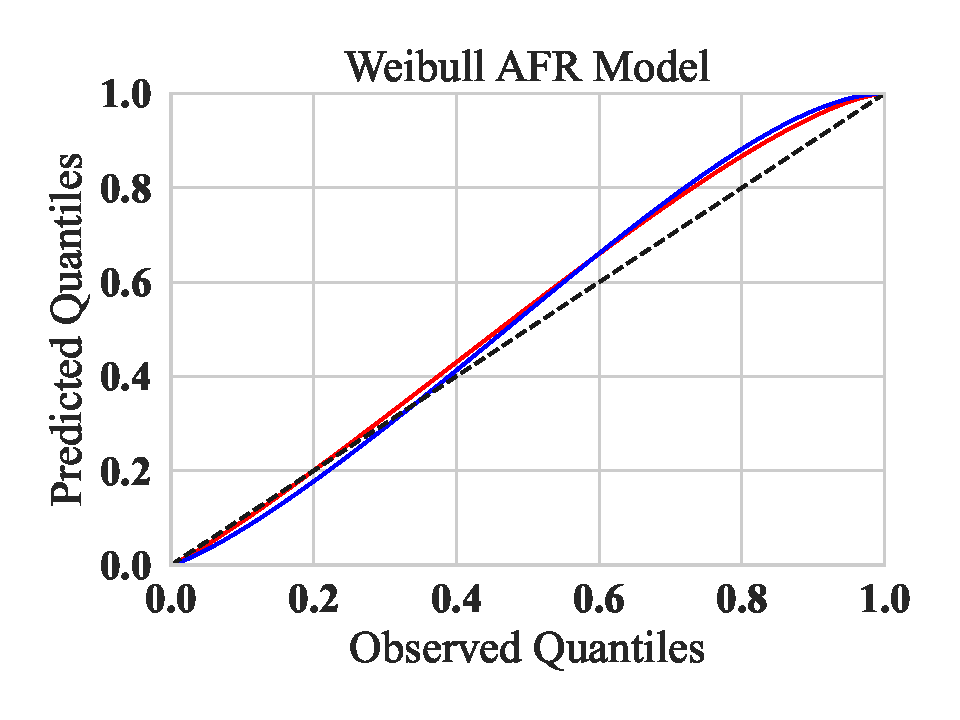
\includegraphics[width=.30\textwidth,trim={20pt 20pt 20pt 20pt},clip]{plots/weibull_qq.pdf}
	\end{subfigure}%
	\begin{subfigure}
		\centering
		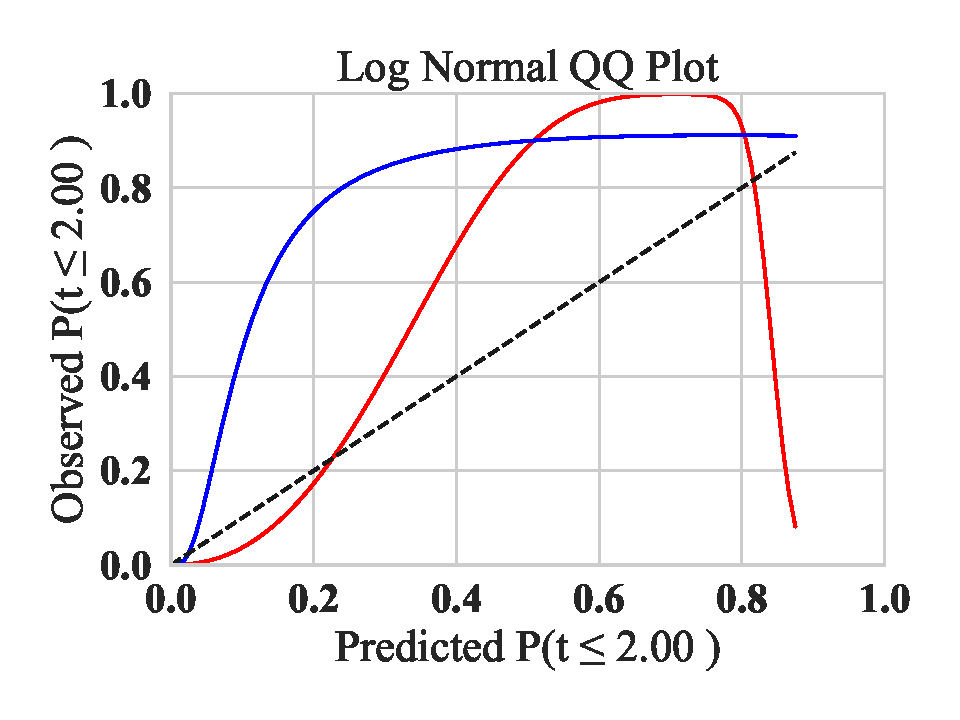
\includegraphics[width=.30\textwidth,trim={20pt 20pt 20pt 20pt},clip]{plots/log_normal_qq.pdf}
	\end{subfigure}
	\begin{subfigure}
		\centering
		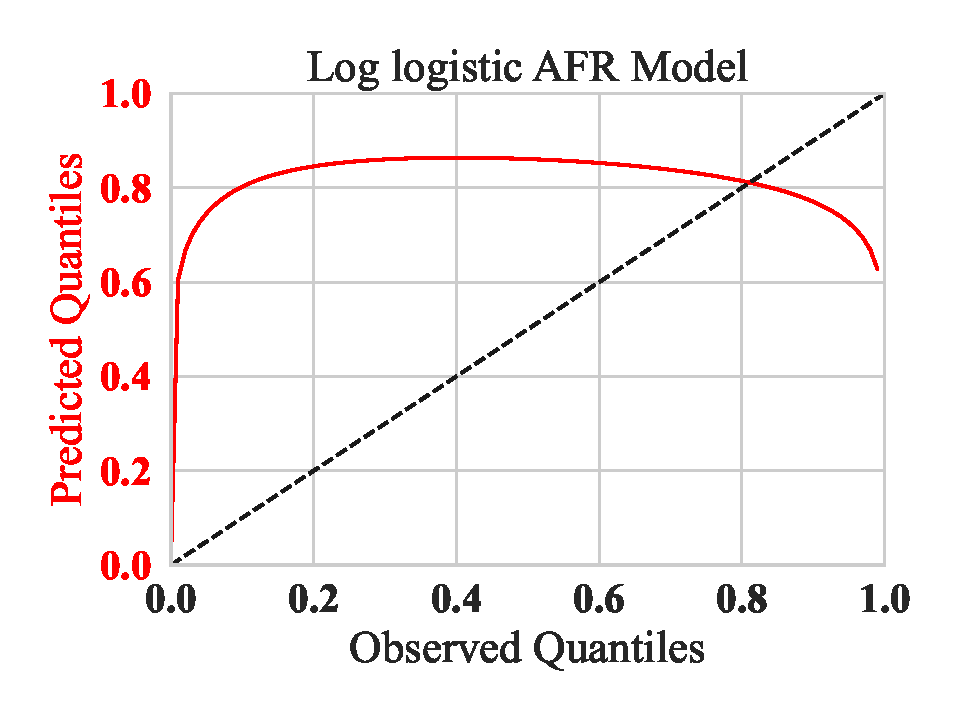
\includegraphics[width=.30\textwidth,trim={20pt 20pt 20pt 20pt},clip]{plots/log_logistic_qq.pdf}
	\end{subfigure}
 \begin{subfigure}
		\centering
		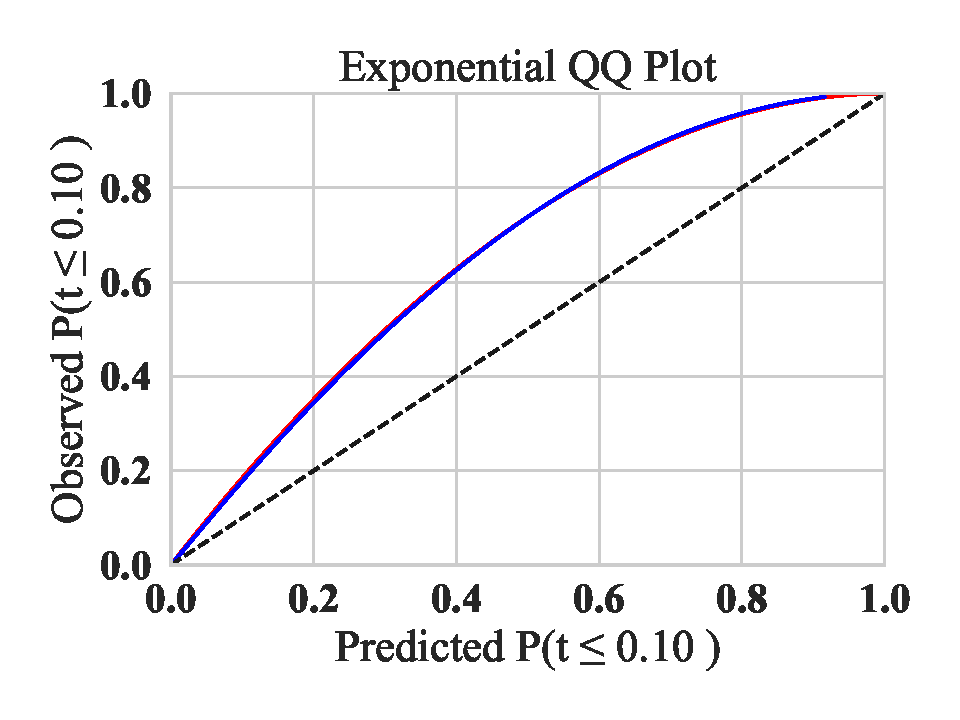
\includegraphics[width=.30\textwidth,trim={20pt 20pt 20pt 20pt},clip]{plots/exponential_qq.pdf}
	\end{subfigure}%
	\begin{subfigure}
		\centering
		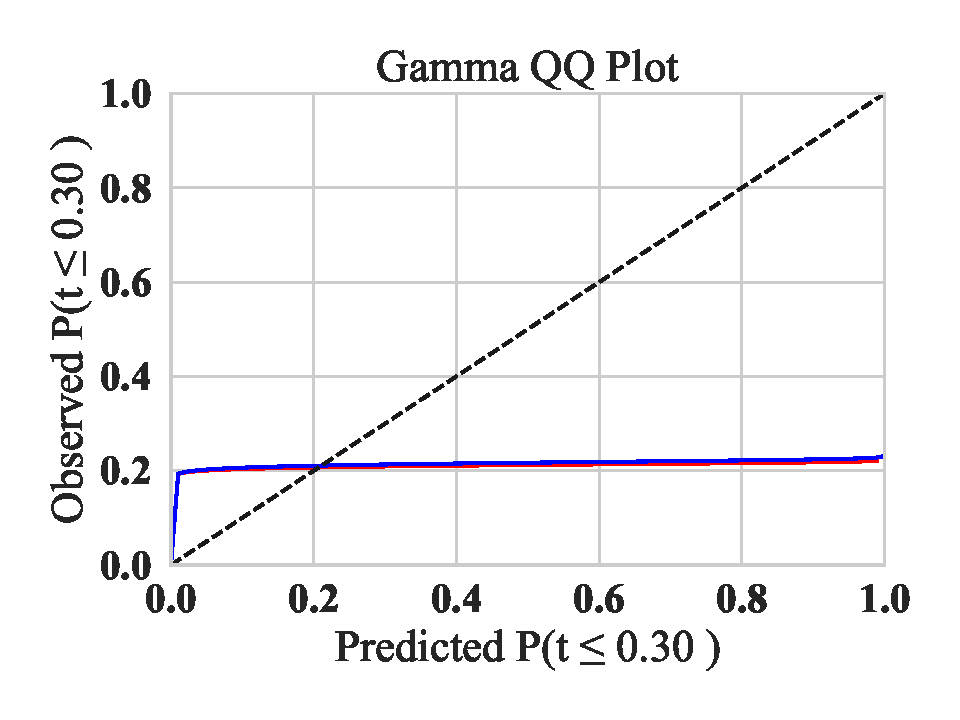
\includegraphics[width=.30\textwidth,trim={20pt 20pt 20pt 20pt},clip]{plots/gamma_qq.pdf}
	\end{subfigure}
	\begin{subfigure}
		\centering
		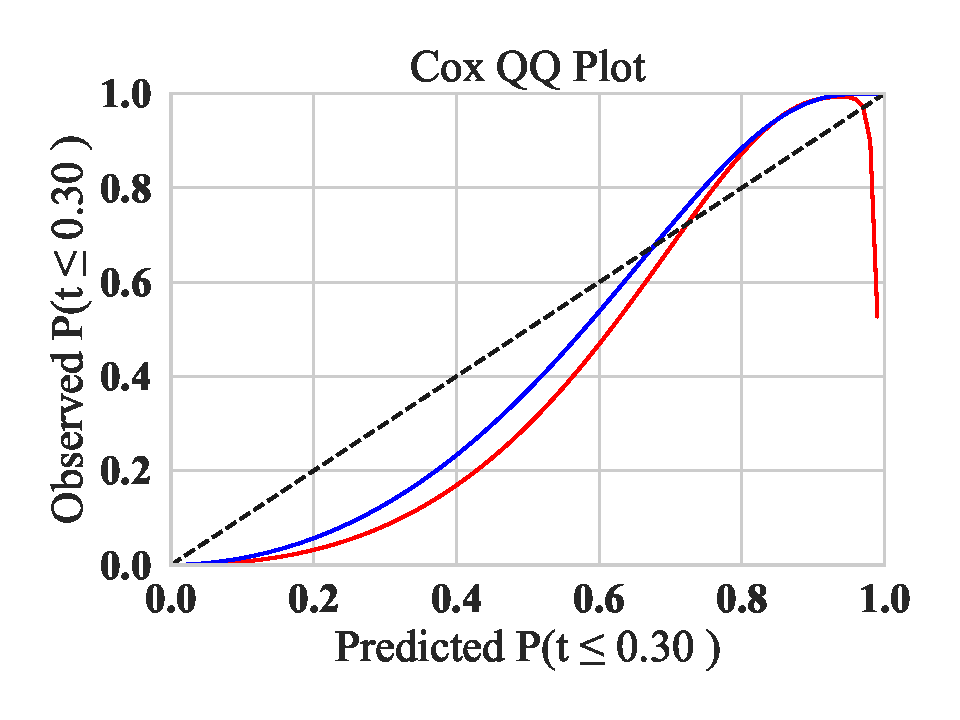
\includegraphics[width=.30\textwidth,trim={20pt 20pt 20pt 20pt},clip]{plots/cox_qq.pdf}
	\end{subfigure}
	\caption{These quantile-quantile plots demonstrate the efficacy of various AFT models. The first axis is the observed quantile of a sample and the second axis represents the theoretical quantile according to the chosen AFT model. The dashed black line represents a perfect fit. To verify each model, we reserved 80\% of the data to be the training set (blue) and 20\% to be the test set (red). The time for each model was chosen to depict the best fit of the curve when $ [ 0 \geq t \leq 10 ] $ seconds.
 % The absence of one of the lines means that the \texttt{lifelines} fitter failed to converge for that subset.
 }
	\label{fig:afr_models}
\end{figure*}

\subsection{Effect of Covariates}
Figure~\ref{fig:dummies} depicts the effect of all attacks, defences, and model configurations on the survival time and Figure~\ref{fig:covariates} depicts the effect of the covariates.
Figure~\ref{fig:covariates} clearly demonstrates that increasing the depth of the model architecture does little for adversarial robustness while universally increasing the training time.
Furthermore, it reveals something surprising -- that increasing the number of epochs tends to increase the failure rate -- even across model architectures and all defences.
Certain defences can outperform the control model -- at the cost of expensive tuning -- evidenced by the large variance in performance (see Figure~\ref{fig:dummies}). The scale of $t_{\mathrm{train}}$  in Figure~\ref{fig:covariates} shows that there is no general relationship between training time and adversarial survival time. Additionally, we see that an increase in accuracy tends to correspond to a decrease in survival time, confirming the inverse relationship noted by many researchers~\cite{carlini_towards_2017,biggio_evasion_2013,croce_reliable_2020}.
As the training time increases, however, the variance of attack times decreases, likely due to the corresponding increase in inference time (see Figure~\ref{fig:covariates}, covariate $t_{\mathrm{predict}}$) rather than inherent robustness (see covariate `Layers').
We formalise this analysis in the next subsection.

\begin{figure}
    \centering
	\begin{subfigure}
	\centering
    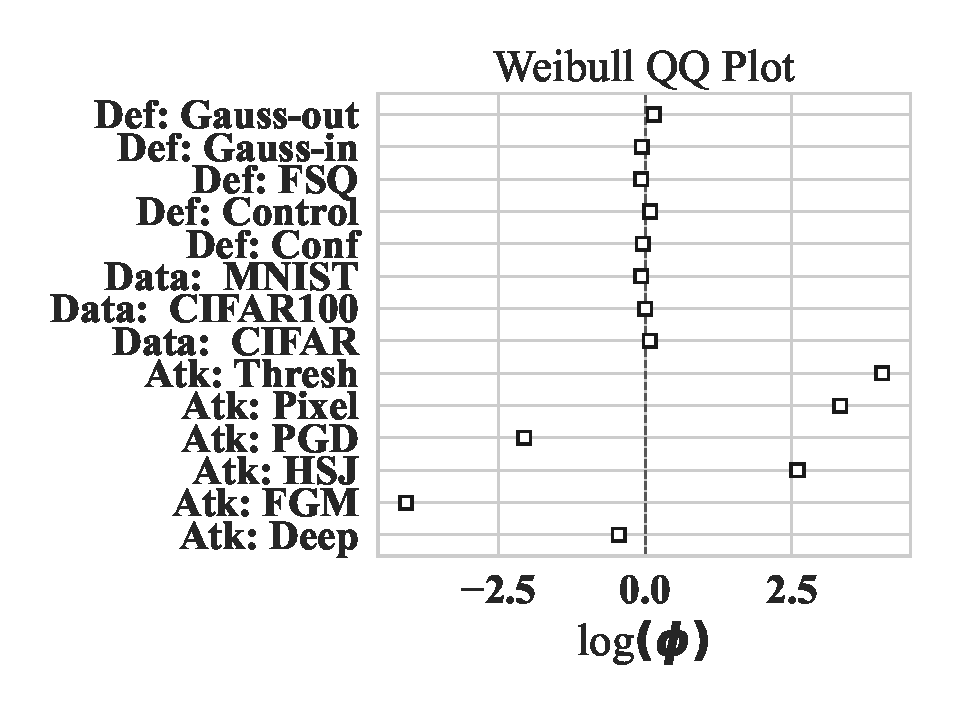
\includegraphics[width=.37\textwidth,trim={25pt 20pt 20pt 10pt},clip]{plots/weibull_aft_dummies.pdf}
    \end{subfigure}
    \begin{subfigure}
	\centering
    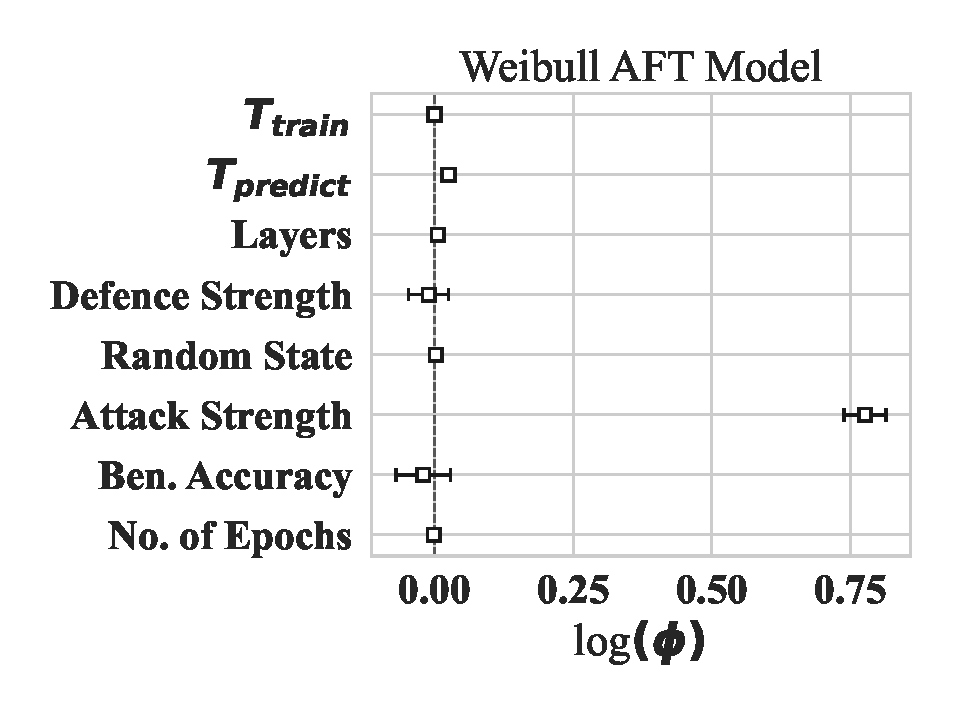
\includegraphics[width=.37\textwidth,trim={25pt 20pt 20pt 10pt},clip]{plots/weibull_aft.pdf}
    \end{subfigure}
    \caption{The coefficients represent the log scale effect of the dummy variables for dataset (Data), attack (Atk), and defence (Def) on the survival time, with a positive value indicating an increase in the survival time. The top plot depicts the covariates and the bottom plot depicts the dummy variables for the different attacks, defences, and datasets.}
    \label{fig:covariates}
    \label{fig:dummies}
\end{figure}


\subsection{Failures and Cost}

Figure~\ref{fig:failures_per_train_time} depicts the cost-failure ratio (see Equation~\ref{eq:cost}) in both the benign (top) figure and adversarial cases (middle and bottom figures), using the Weibull model to calculate $\mathbb{E}[T]$. Counter-intuitively, we see that the smallest model (ResNet18) tends to outperform both larger models (ResNet50 and ResNet152). Furthermore, we see that defence tuning is about as important as choosing the right type of defence (see left side of Figure~\ref{fig:failures_per_train_time}), with all defences falling within the normal ranges of each other. However, adding noise to the model output (Gauss-out) tends to underperform relative to the control for all models (see left side of Figure~\ref{fig:failures_per_train_time}). Likewise, the efficacy of a defence depends as much on model architecture as it does on hyperparameter tuning as demonstrated by the large variance in Figures~\ref{fig:accuracies}~\&~\ref{fig:failures_per_train_time}.  Furthermore, performance across all attacks is remarkably consistent with intra-class variation being smaller than inter-class variation almost universally across defences and model configurations.
Finally -- and most importantly -- we see that every single tested configuration performs incredibly poorly against FGM and PGD\@.

\begin{figure}[!ht]
    \centering
    \begin{subfigure}
        \centering
        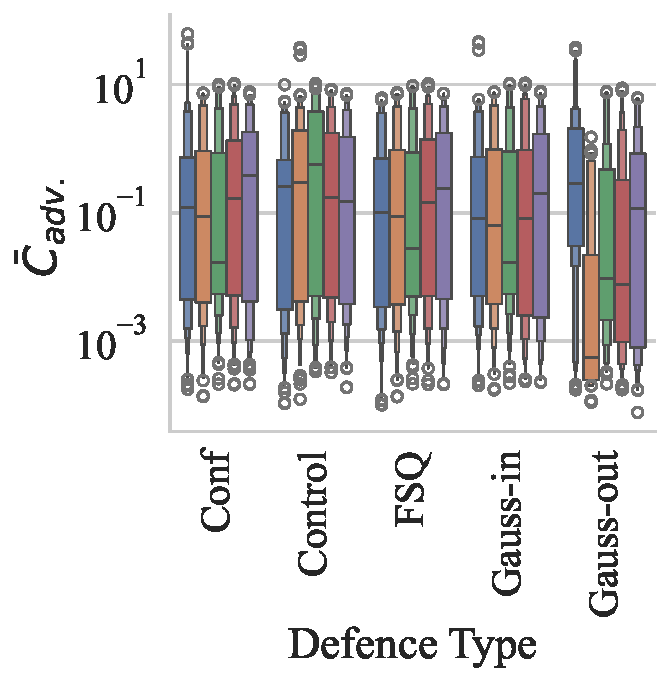
\includegraphics[width=.38\textwidth,trim={12pt 10pt 20pt 10pt},clip]{plots/trash_score_vs_defence_type.pdf}
    \end{subfigure}
    \begin{subfigure}
        \centering
        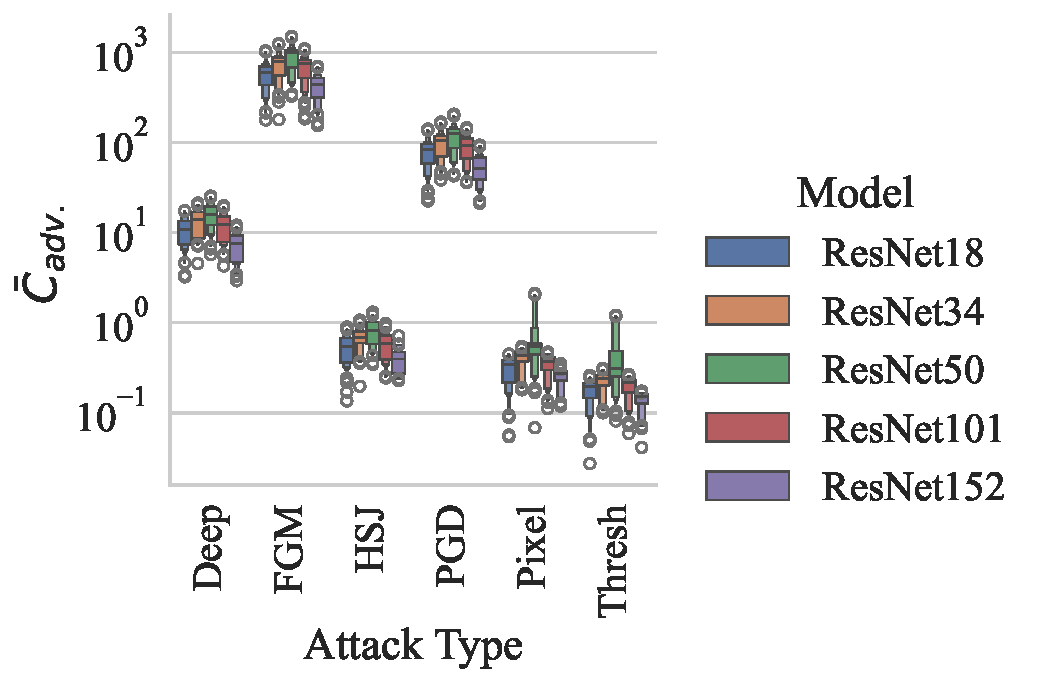
\includegraphics[width=.38\textwidth,trim={12pt 10pt 20pt 10pt},clip]{plots/trash_score_vs_attack_type.pdf}
    \end{subfigure}
    \caption{This figure depicts the TRASH metric that reflects the ratio of training-to-attack times, where a value$\gg 1 $  indicates an essential advantage for the attacker. The violin plots reflect the 95\% confidence intervals for each tuned hyperparameter combination. Outliers are indicated with a circle.}
	\label{fig:failures_per_train_time}
\end{figure}